\section{Monad}\label{sec:standardmonad}
Now we come to the module \verb\Monad\.
This module takes a mathematical concept and makes into practical programming construct.

First we are going to look at what monads exactly are within programming.
Then we will see how they are implemented within MC.

\subsection{Monads}
Monads are a container like, generic interface.
They contain two functions:

\begin{itemize}
   \item Return
   \item Bind
\end{itemize}

These two functions create the basis on which the monads are built.

\subsubsection{The return}
The return function takes a value and wraps it inside a monad.

{
   \centering
   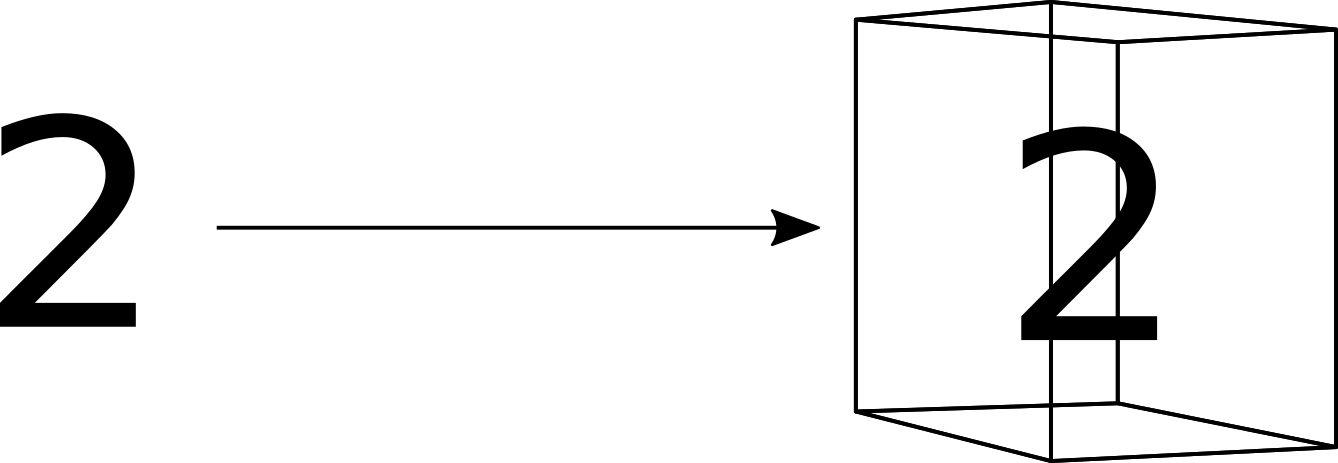
\includegraphics[width=\columnwidth]{return}\\
   \captionof{figure}{The return}\label{fig:monadreturn}
}

The box in figure~\ref{fig:monadreturn} visualizes the monad and \verb\2\ is the value that is being put inside the monad.
With the return function any value can be put inside a monad.
When it is inside the monad it cannot be seen by the outside world.

This is where the bind comes in.

\subsubsection{The bind}
Having a monad is fine, but what if you want to manupilate the value of the monad?
The bind function supplies this functionality.

{
   \centering
   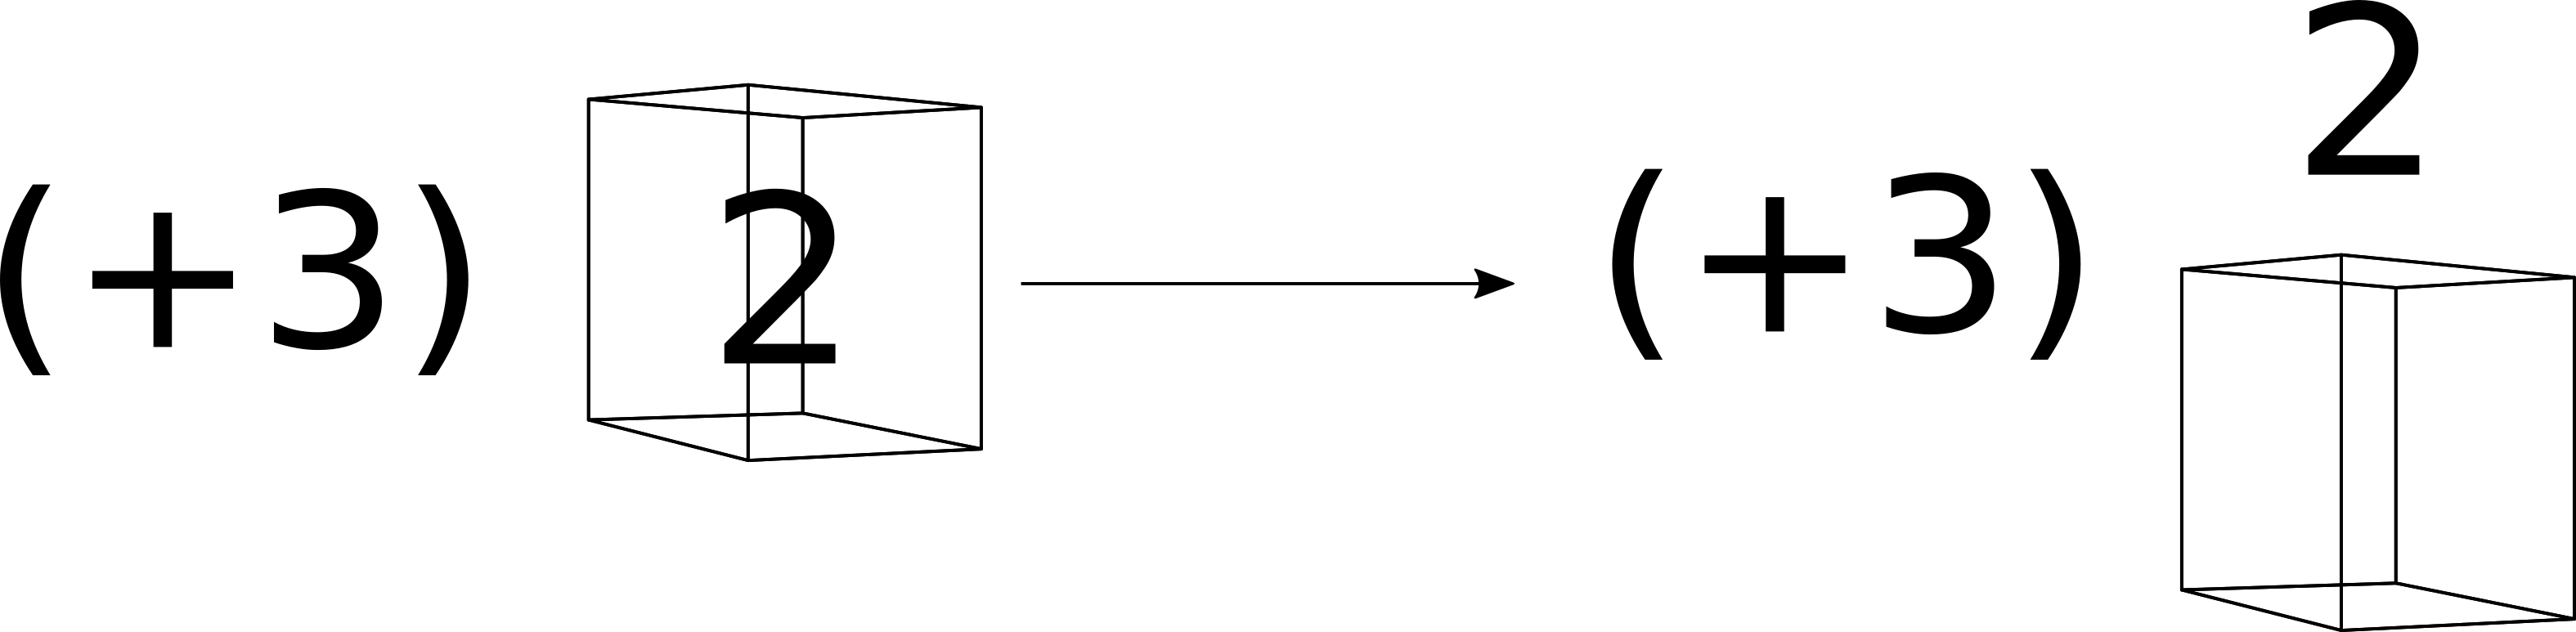
\includegraphics[width=\columnwidth]{bind1}\\
   \captionof{figure}{A function and a monad}\label{fig:monadreturn}
}

When we want to apply the function \verb\(+3)\ to the monad containing \verb\2\, we call the bind.
The bind unpacks the monad.

{
   \centering
   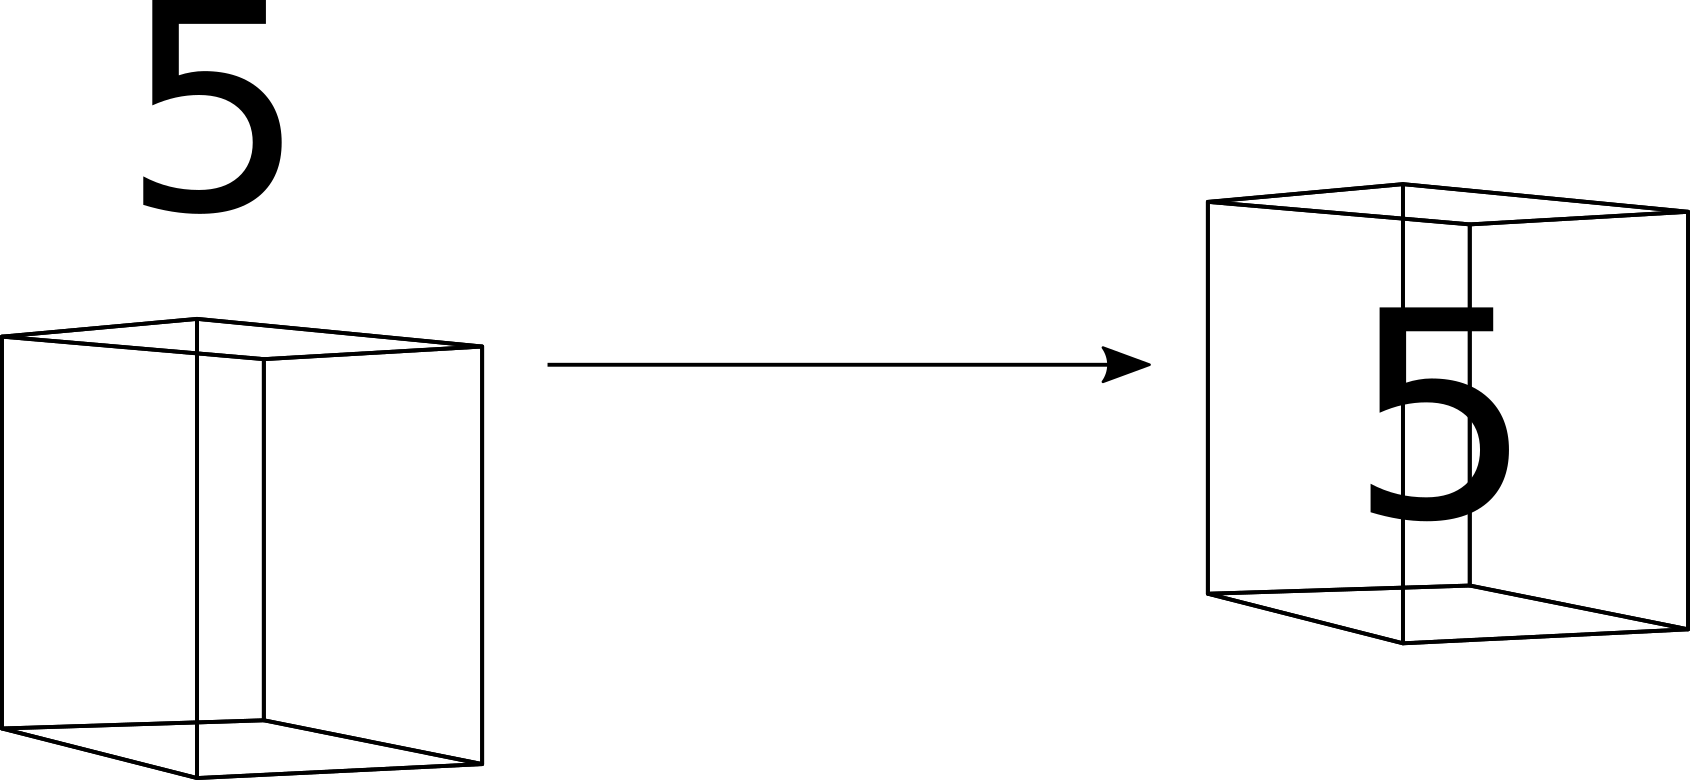
\includegraphics[width=\columnwidth]{bind2}\\
   \captionof{figure}{The return}\label{fig:monadreturn}
}

Applies the function to the value.
And then packs the new value inside the monad.

Using these two basic functions, we can always work with monads.
The monads have then become the generic interface of every function.
This gives us greater safety when moving values between functions, because the values thrown between functions are always monads.

\subsubsection{More than a wrapper}
But just a monad offers very little besides being a wrapper for values.
That is why there have been created a few different sorts of monads.

We will discuss two of these for now.
More will be explained when looking at the implemented monads in MC, see section~\ref{sec:standardimplementedmonads}.

\paragraph{The state monad}
gives monads the ability to behave like mutables.
It takes a \emph{state} and returns a new state and a return value.

Say we want to roll a dice.
The state monad will simulate the \emph{state} of the dice being roled.
The state monad is given a \emph{state} of the dice and from this it will compute the new state of the dice and the number roled.

In MC the functionality might look like this:

\begin{lstlisting}
Func "state" -> 's -> ('a,'s)
state dice -> (numberRoled,newDice)
\end{lstlisting}
MAYBE LEAVE IT IN BUT PROBABLY BEST TO LEAVE CODE OUT OF STATE MONAD FOR NOW.


\paragraph{The maybe monad}
offers the ability of the value to be either a value or nothing.
For example we could utilize the pipe operator for this:

\begin{lstlisting}
Data "Maybe" -> 'a -> 'a | Unit

Func "test" -> Maybe -> Boolean^System
(match a with
  (\ x -> True^builtin)
  (\ unit -> False^builtin)) -> res
-----------------------------------
test a -> res
\end{lstlisting}

Here we use \verb\Unit\ as the nothing and 'a as the value.
In the example the term a is checked for a being a value, the \verb\Left\, or being nothing, the \verb\Right\.

This is a very basic example of how the maybe works.
It acts like a pipe and can contain either a value, \verb\Left\, or nothing, \verb\Right\.

\subsubsection{Combining monads}
Apart from having different sorts of monads, they can also be combined.
Since they are the same generic interface they can be combined into another generic inteface.
These new monads can utilise the functionality of the all combined monads.

In this manner the functionality of a monad can be extended.

{
   \centering
   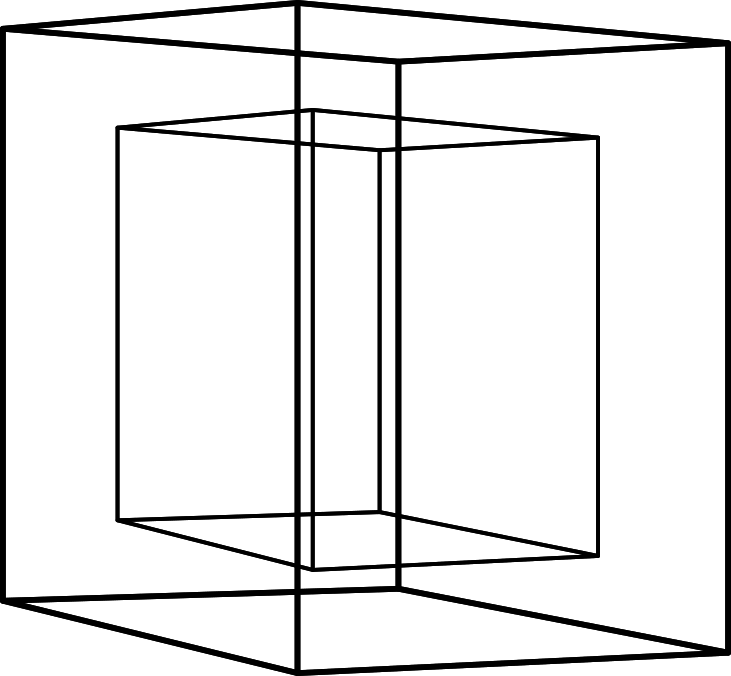
\includegraphics{transformers}\\
   \captionof{figure}{Combining monads}\label{fig:monadcombining}
}

Combining monads can be seen as putting one monad inside another monad, as illustrated in figure~\ref{fig:monadcombinig}.

We will take the state and maybe monad and combine these into a parser monad.
A parser monad can parse through a data structure and scan for certain elements.

The state monad will be used for the scanning functionality and the maybe monad will be used to determine of the elemnt has been found.
The state monad returns the maybe monad as its result.
When the maybe monad has a value as result the parser monad stops.

Like the normal monads they have to be build manually.
This is a very error prone process when combining more than two monads or when using more complex monads.

What we actually want is to write the monads once and use combine them automatically.
This is where monad transformers come in.

\subsection{Monad transformers}
Monad transformers are a way to automatically combine monads.
Instead of simply having a monad which takes the arguments it needs, it also takes another monad transformor as one of its arguments.
This monad transformer is then used to wrap the result.

Combining monads this way is quite useful when having complex monads.
Because the combining happens naturally with monad transformers, there are no errors created in the process of combining.

MC has an implementation of the basic monad transformer with which all monad transformers can be created.

\subsection{Implementation}\label{sec:basicmonadsimplementation}
Now we will look at how the monad transformer is implemented.
With this monad transformer we will be able to create actual monads, this can be seen as the basic interface of a monad.

First we take a look at the declaration:

\begin{lstlisting}
TypeFunc "Monad" => (#a => #b) => Module
\end{lstlisting}

Monads are implemented as modules.
This way we can put the return and bind functions inside a monad.

The first argument is a function on type level.
It represents the monad transformer it uses to wrap the result in.

When looking at the implementation we see that a module is created with the return and the bind:

\begin{lstlisting}
Monad 'M => Module {
  ArrowFunc 'M 'a -> ">>=" -> ('a -> 'M 'b) -> 'M 'b   #> 10
  Func "return" -> 'a -> 'M 'a
\end{lstlisting}

The bind is declared with \verb\ArrowFunc\ and is called \verb\>>=\.
It takes a monad as its first argument and the function to create the new monad as its second argument.
It returns the monad created with the function it takes.

The return takes a value, \verb\'a\, and wraps it inside the monad, \verb\'M\.

Both the bind and the return are only declared and not defined, because they are different for every monad created.
When creating a new monad the bind and return will need to be defined.

Sometimes we want to directly pass the value inside the monad instead of wrapping it.
This is done with \verb\returnFrom\.

\begin{lstlisting}
  Func "returnFrom" -> 'a -> 'a
  returnFrom a -> a
\end{lstlisting}

This function can be defined in the monade interface, because it is the same for every monad.

Next we need to know the signature of the monad wrapped inside the monad created.

\begin{lstlisting}
  TypeFunc "MCons" -> #a
  MCons -> 'M
\end{lstlisting}

This is needed when declaring new functions which utilise the wrapped monad.

Then we have the lift functionality.

\begin{lstlisting}
  Func "lift" -> ('a -> 'b ) -> 'M 'a -> 'M 'b
  {a >>= a'
     return f a'} -> res
  ----------------------
  lift f a -> res
\end{lstlisting}

The \verb\lift\ takes a regular function, that goes from one value to another, and a monad.
This monad is then unwrapped, \verb\a >>= a'\, and the value is passed to the function, \verb\f a'\.
The result of this is then wrapped again inside the monad and returned with the monadic \verb\return\.

The \verb\Lift\ can also be declared with functions which take two arguments.

\begin{lstlisting}
  Func "lift2" -> ('a -> 'b -> 'c) -> 'M 'a -> 'M 'b -> 'M 'c
  {a >>= a'
     b >>= b'
       return f a' b'} -> res
  ---------------------------
  lift2 f a b -> res
\end{lstlisting}

This can be expanded to functions which take any number of arguments.

There are ofcourse functions which work with the wrapped monad.
For this \verb\liftM\ is created.

\begin{lstlisting}
  Func "liftM" -> (MCons^'M 'a -> MCons^M' 'b) -> 'M (MCons^'M 'a) -> 'M (Mcons^'M 'b)
  {M >>=^'M a
    f a -> b
    return^'M b} -> res
  ---------------------
  liftM f M -> res
}
\end{lstlisting}

It works the same as the other lift functions, with the specification of using the bind and return of the wrapped monad, \verb\'M\, instead of the bind and return of the current monad.

Now we have the complete interface of the monad transformer.
With this we can combine and built monads automatically.


\subsection{Evolution}


\section{TryableMonad}
Apart from the regular monadic interface there is also the tryable monadic interface.
This creates a monad with a few extra functions, namely the \emph{try}.

It uses the regular monadic interface to create a new interface.

\begin{lstlisting}
TypeFunc "TryableMonad" => (#a => #b) => Module
TryableMonad 'M => Monad(MCons^'M) {
  inherit 'M
\end{lstlisting}

As declared \verb\TryableMonad\ takes a monad as its argument and creates a new module.
It uses the type signature of \verb\'M\ to create a new monad and inherits the functions from \verb\'M\.

Here we also see the first use of \verb\MCons\.
When creating monads using other monads this function comes in very handy.

Then we declare the \verb\try\ function and initialise \verb\e\.

\begin{lstlisting}
  Func "try" ('a -> MCons^'M 'b) => ('e -> MCons^'M 'b) => MCons^'M 'a => MCons^'M 'b
\end{lstlisting}

If \verb\try\ succeeds the first function will be executed and if it fails the second function will be executed.

We also want to be able to get the original monad out of the tryable monad.
This is done with \verb\getMonad\.

\begin{lstlisting}
  $$ return the monad of the tryable monad, this way you can use the tryable monad as a the normal monad
  Func "getMonad" -> MCons^'M
  getMonad -> 'M
}
\end{lstlisting}

Here the original monad is given when \verb\getMonad\ is called.

\subsection{Evolution}

\section{Implemented monads}\label{sec:standardimplementedmonads}
\subsection{Id}\label{sec:basicmonadsimplementedid}
The main problem with using monad transformers is that the always take another monad.
There is no end to the chain.

That is why we have the \emph{id} monad transformer.
It takes no monad as argument and simply returns all values as the are.

First wee need a type signature to tell the monad interface which monad we are creating.

\begin{lstlisting}
TypeAlias "Id" => #a => #b
Id 'a => 'a
\end{lstlisting}

Here we can see what the id monad should do, simply pass the type on as it was given.

Now we will declare and define the id monad:

\begin{lstlisting}
TypeFunc "id" => Monad
id => Monad(Id) {
  bind x k -> k x
  return x -> x
}
\end{lstlisting}

Here we see how the monad transformer interface in called and instantiated with the type signature created with \verb\Id\.

\verb\Id\ also takes a \verb\'a\, but this is never used as the id monad does not need an extra type to say which type it really uses.
While the \verb\'a\ is not used, it necessary to have them in the type signature.
Else \verb\Id\ cannot be used to instantiate \verb\Monad\, as evident from section~\ref{sec:basicmonadsimplementation}.

Other monad transformers which do actually use the \verb\'a\ also do not instantiate them immediatly.
The programmer can decide for which type the monads will be created, therefor it is left open.
This effectively creates an interface for the defined monad to be instantiated with a type later specified.

The \verb\return\ simply returns the exact same value and \verb\bind\ executes the function \verb\k\ with \verb\x\ as its argument.

When using the \verb\id\ monad transformer with another transformer, it becomes that monad.
Because the values are directly returned from the \verb\id\ transformer the values are directly used in the other monad transformer, thus creating that monad.


\subsection{List}
The list monad is a monad with a list inside itself.

First we needed to create a list that can work with types.

\begin{lstlisting}
TypeAlias "List" => #a => Unit | (#a * (List #a))
List unit => Left unit
List 'a => Right ('a * (List 'a))
\end{lstlisting}

It uses the pipe operator to create \verb\List\.
This is necessary because we need an end to the list, which in this case is \verb\Unit\.
In \verb\Right\ the list is created recursively with the help of a tuple.

We also need the basic operators to create lists.

\begin{lstlisting}
TypeAlias #a -> "::" -> List -> List
'a :: 'b => List ('a * 'b)

TypeAlias "empty" -> List
empty => List unit
\end{lstlisting}

A list can now be created with the \verb\::\ operator.
We can also intatiate an empty list with \verb\empty\.

But we would also like to concat lists together.

\begin{lstlisting}
Func List 'a -> "@" -> List 'a -> List 'a  #> 200
empty @ l -> l
(x :: xs) @ l -> x :: (xs @ l)
\end{lstlisting}

This is done with the \verb\@\ operator.

And when we want to apply a function to the entire list we call \verb\map\.

\begin{lstlisting}
Func "map" -> List 'a -> ('a -> 'b) -> List 'b
map empty f -> empty
map (x :: xs) f -> (f x) :: (map xs)
\end{lstlisting}

This executes a function and creates a new list, which it then returns.

When we want to find one or more elements in the list we can call \verb\filter\.

\begin{lstlisting}
Func "filter" -> List 'a -> ('a -> Boolean^System) -> List 'a
filter empty p -> empty

(if p x then
  (x :: (filter xs p))
  else
  (filter xs p)) -> res
-------------------------
filter (x :: xs) p -> res
\end{lstlisting}

The programmer still has to create the function that actually does the checking, but \verb\filter\ checks the entire list and returns a new list.
The returned list contains the elements which are specified in function \verb\p\.

Now that we have the complete \verb\List\ type defined and its functions, we can create the actual monad.
First we have to declare and define the list monad signature.

\begin{lstlisting}
TypeAlias "ListT" => (#a => #b) => #c => #d
ListT 'M 'a => 'M(List 'a)
\end{lstlisting}

Using \verb\ListT\ together with the signature of \verb\'M\ we create the \verb\list\ monad.

\begin{lstlisting}
TypeFunc "list" => Monad => Monad
list 'M => Monad(ListT MCons^'M) {
\end{lstlisting}

\verb\ListT\ also takes a \verb\'a\, which is the type for the list created.
As stated in section~\ref{sec:basicmonadsimplementedid} it will be left up to the programmer to do this.

When we look at the return it simply puts the value in a list and packs it into the monad.

\begin{lstlisting}
  return x -> return^'M(x :: empty)
\end{lstlisting}

The bind looks a bit more complicated.

\begin{lstlisting}
  {lm >>= l
    (match^prelude l with
      (\empty -> return^'M empty)
      (\(x :: xs) ->
        {x >>=^'M y
          return^'M k y} -> z
        xs >>= k -> zs
        (z @ zs)))} -> res
  -------------------------------
  lm >>= k -> res
}
\end{lstlisting}

It starts with the \verb\ArrowFunc\ syntax and uses the match to determine if the list actually contains a list or not.
When it is \verb\empty\ the bind simply returns an empty.

When a list is present the first element of the list gets unpacked by the bind of \verb\'M\, which gets named \verb\y\.
The function \verb\k\ gets executed with \verb\y\ as its argument and the result gets repacked by the return.

Now the rest of the list, \verb\xs\, gets passed to the bind of \verb\list\ so the entire list gets passed to \verb\k\.
The results of processing \verb\x\ and \verb\xs\ are then concatenated into a single list which gets returned as a result of the bind.

If the use of the different syntaxes of the \verb\ArrowFunc\ seems confusing, take extra look at section~\ref{sec:basicmcarrowfunc}.

\subsubsection{Evolution}
\subsection{Either}\label{sec:basicmonadseither}
The either monad is an implementation of the \verb\TryableMonad\ interface.

It creates a monad which can be either a value or a list of fails.
The type signature is as follows:

\begin{lstlisting}
TypeAlias "EitherT" => (#a => #b) => #c => #d => #e
EitherT 'M ['e] 'a => 'M('a | 'e)
\end{lstlisting}

It uses the pipe to be able to be either failed or a value.

The \verb\Tryable monad\ is then called with the signature of the monadic argument.

\begin{lstlisting}
TypeFunc "either" => Monad => #a => TryableMonad
either 'M (List 'e) => TryableMonad(EitherT MCons^'M (List 'e)) {
\end{lstlisting}

The \verb\'a\ is again not used, as is complient with section~\ref{sec:basicmonadsimplementedid}.

Next we see the bind and return defined:

\begin{lstlisting}
  pm >>= k -> try pm k fail
  return x -> return^'M(Left x)
\end{lstlisting}

The bind calls \verb\try\ which is declared but not yet implemented.
The try will then be defined:

\begin{lstlisting}
  {pm >>=^'M y
    (match y with
      (\x -> k x)
      (\e -> err e)) -> z
    return^'M z} -> res
  ---------------------
  try pm k err -> res
}
\end{lstlisting}

The \verb\try\ takes monad, a function and an error function.
The error function will be executed if \verb\y\ contains an error and if it contains a value the first function will be executed.

It calls the bind if \verb\'M\ to get to the value inside.

We also have a fail function which can be called if the monad fails.

\begin{lstlisting}
  Func "fail" -> 'e -> MCons 'b
  fail e -> return^'M(Right (Right^'M :: e))
\end{lstlisting}

What these fails are is up to the programmer.
The fails get concatinated into a list and returned.

\subsubsection{Evolution}
\subsection{Option}
CAN THIS BE LEFT OUT???????????
probably yes

\begin{lstlisting}
TypeFunc "Option" => #a => #b
Option 'a => Unit | 'a

Func "Some" -> 'a -> Option 'a
Some x -> Right x

Func "None" -> Option 'a
None -> Left Unit

TypeFunc "option" => TryableMonad
option => either Option None {
  return
}
\end{lstlisting}
\subsubsection{Evolution}

\subsection{Result}
The result monad is complete implementation of the either monad from section~\ref{sec:basicmonadseither}.
It takes a monad and uses a \verb\String\ as the error type.

\begin{lstlisting}
TypeFunc "result" => Monad => TryableMonad
result 'M => either MCons^'M (List String)
\end{lstlisting}

\subsubsection{Evolution}
\subsection{State}
We have hade a basic explanation of the state monad in section~\ref{sec:standardmonad}.

Now we will see how it is really implemented.
The first thing to do is create a type signature of the state monad:

\begin{lstlisting}
TypeAlias "StateT" => (#a => #b) => #c => #d => #e
StateT 'M 's 'a => ('s -> 'M('a * 's))
\end{lstlisting}

As we can see the state monad is defined as a function.
It takes a state and returns a monad containing a tuple af the resulting value and the new state.

We use \verb\StateT\ in the call to \verb\Monad\ so it knows what the type signature will be.

\begin{lstlisting}
TypeFunc "state" => Monad => #a => Monad
state 'M 's => Monad(StateT MCons^'M 's) {
\end{lstlisting}

When looking at the return we see something new.

\begin{lstlisting}
  return x -> (\ s -> return^'M(x,s))
\end{lstlisting}

A lambda is created to match the type signature of the state monad.

We see this happening also in the bind.

\begin{lstlisting}
  (\ s ->
    {p s >>=^'M x
      x -> (x',s')
      k x' s'}) -> res
  ---------------------
  p >>= k -> res
\end{lstlisting}

The bind of \verb\'M\ is called and the result is then deconstructed to get to the tuple which it contains.
We know \verb\x\ is a tuple because it lives inside a state monad which always creates a tuple inside the resulting monad.
As is evident by the type signature of the state monad.

The state monad also contains two extra functions.
They make it possible to get and set the state.

To get the state we call \verb\getState\.

\begin{lstlisting}
  Func "getState" -> MCons 's
  getState -> (\ s -> return^'M(s,s))
\end{lstlisting}

It sets the state as the result in the return lambda.
By which you will get the state back when it is entered into the lambda.

To set the state we call \verb\setState\.

\begin{lstlisting}
  Func "setState" -> 's -> MCons Unit
  setState s -> (\ unit -> return^'M(unit,s))
}
\end{lstlisting}

It sets the result to unit and the state to the input state.

\subsubsection{Evolution}
\subsection{IO}
\subsubsection{Evolution}
